\chapter[Semi-supervised binary classification]{Semi-supervised binary classification of animate and inanimate objects}
\label{chap:bmt-exp} % id kapitoly pre prikaz ref

In this chapter, we focused on the existing model Binary mean teacher, which is derived from the semi-supervised model Mean Teacher, and is used for binary classification. Our task was to classify images of animate and inanimate objects. We used images from the standard CIFAR-10 image dataset. The main goal of this experiment was to test the performance of the Binary mean teacher model in yet unstudied conditions. We have done several hyperparameter experiments with this new dataset and compared semi-supervised model performance with a supervised baseline.


\section{Task description}

Our goal was to find out, whether the model can discover features that are specific to the appearance of living creatures and others that define lifeless objects and differentiate these two classes of objects. Simply, our task was the classification of images into two classes - animate objects and inanimate objects. For this task, we needed a dataset, that contains images from both categories. We chose the CIFAR-10 dataset, which is a standard dataset for multi-class classification. We relabeled the samples to comply with our task.


\section{Modification of CIFAR-10 dataset}
\label{dataset-cifar10}

We chose to transform and use standard CIFAR-10 dataset \cite{krizhevsky2009} which consists of $60\,000$ color images with resolution $32 \times 32$ pixels in $10$ classes (bird, cat, deer, dog, frog, horse, airplane, automobile, ship, truck), with $6\,000$ images per class. 

In this experiment, we transformed the dataset from the original ten classes into two - animate and inanimate. The animate class was formed of images from the original classes bird, cat, deer, dog, frog and horse. The inanimate class consisted of images that were originally in classes airplane, automobile, ship and truck. Examples of images from the dataset are shown in figure \ref{fig:cifar10}.

Then we split the dataset into training and test sets. The test set was formed from $10\,000$ samples. The training set has unlabeled and labeled part, which are formed by the rest of the data. The proportion of labeled samples was the subject of experimentation.

\begin{figure}[h!]
    \centering
    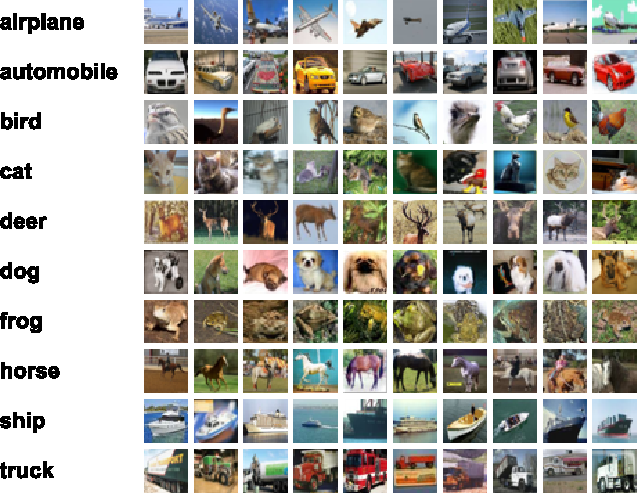
\includegraphics[width=0.9\textwidth]{figs/cifar10-sample-fig.pdf}
    \caption{Example images from CIFAR-10 dataset classes}
    \label{fig:cifar10}
\end{figure}

\section{Models}

We compared the semi-supervised model performance with the supervised model to show, how the unsupervised part of the model supports learning. As far as the task was designed for binary classification, we decided to use the semi-supervised model Binary mean teacher described in section \ref{bmt}. As a supervised baseline we used multi-layer perceptron \ref{mlp} with the same layer architecture as a semi-supervised model. 
 
The architecture of hidden layers was taken from Sarmad's Github repository \cite{sarmad-repo}, from his implementation of the Mean Teacher model. The neural network had $25$ hidden convolutional and batch normalizing, dropout and pooling layers described in table \ref{layers} with ReLU as activation functions for all layers except the last two. In the last two layers, the sigmoid activation function was used.


\subsection{Semi-supervised BMT model}
The core of the model implementation was taken from Sarmad's Mean Teacher implementation \cite{sarmad-repo}. We used his hidden architecture but changed the last layer dimension to $1$, which is a more suitable representation for binary classification. We also changed the unsupervised loss (MSE) calculation to use representation from the last convolution layer instead of network output, because network output is a single number, which does not contain much information. Supervised loss computation function was changed from Cross entropy to Binary cross entropy loss function, for the same reason. These changes were sufficient to transform the Mean Teacher into the Binary mean teacher model. 

During development, we found out, that using feature vectors from the last convolutional layer when computing MSE is essential for network convergence. 

\bigskip

\begin{table}[ht]
    \centering
    \begin{tabular}{ |l|r|r|} 
     \hline
            Hidden layer type & Size / Kernel size & Parameters\\
            \hline
            3 $\times$ BatchNorm2d &  & \\
            \hline
            3 $\times$ Conv2d & kernel size = 3 & padding = 1 \\
            \hline
            MaxPool2d & kernel size = 2 & stride = 2\\
            \hline
            Dropout & & p = 0.5\\
            \hline
            3 $\times$ BatchNorm2d &  &\\
            \hline
            3 $\times$ Conv2d & kernel size = 3 & padding = 1 \\
            \hline
            MaxPool2d & kernel size = 2 & stride = 2\\
            \hline
            Dropout & & p = 0.5\\
            \hline
            3 $\times$ BatchNorm2d &  & \\
            \hline
            Conv2d & kernel size = 3 & \\
            \hline
            2 $\times$ Conv2d & kernel size = 1 & \\
            \hline
            AvgPool2d & kernel size = 6 & stride = 6\\
            \hline
            nn.Linear & size = 128 &\\
            \hline
            BatchNorm1d & & \\
     \hline
    \end{tabular}
    \caption{Hidden layers of model}
    \label{layers}
\end{table}


\subsection{Supervised baseline}
Our baseline was a deep network trained on the same portion of labeled data. We used a fully supervised multi-layer perceptron and computed accuracy on our custom-modified dataset. As we mentioned, this network had the same architecture as the student or teacher network, so the difference in accuracy should show the effect of using additional information from unsupervised loss in the learning of a semi-supervised model. 

\subsection{Implementation repository}
The implementation of models and the whole experiment was developed in our GitHub repository \cite{dt-mt-repo}. The location of the code for this experiment is in folder \\ \texttt{pytorch/experiments/bmt-animacy}. The folder contains code for dataset transformation and training and evaluation of the Binary mean teacher model and baseline.


\section{Experimental results}
We ran 3 experiments, each oriented on a different hyperparameter investigation. The first one focused on the learning rate hyperparameter, which gives good results for a semi-supervised model. The second discovered how different types of augmentation influence model accuracy, and the last one was about trying different amounts of labeled data in the training set and looking at whether unlabeled data which semi-supervised model use helped its performance in comparison to the supervised model with only labeled data.

\label{bmt:training}
We trained all networks for $30$ epochs and used Adam optimizer. The ratio of labeled and unlabeled samples in the training set was constant and was $4\,000:46\,000$. The network was evaluated on $10\,000$ labeled samples. As image augmentations, we used random flipping and rotations.

For the following two experiments, we trained the baseline on $4\,000$ labeled training samples Learning rate was set to $0.5$, optimizer was Adam. The best accuracy that the network achieved was \textbf{93\%}, as evaluation on $10\,000$ labeled samples.

\subsection{Experiment 1: Learning rate}
We tried several values of the learning rate hyperparameter and trained only a semi-supervised model with other parameters set as described in section \ref{bmt:training}. Our goal was to observe, which values of learning rate were good for the task. 

The best achieved accuracies of the model we get were \textbf{91\%}, with learning rate $0.5$, $89\%$ with learning rate $0.1$ and $87\%$ with learning rate $0.05$.  In the following experiments, we used two best values of learning rate - $0.5$ and $0.1$ in the investigation of different parameters. We can see, that the best accuracy of the BMT model was not higher than the accuracy of the baseline.

\subsection{Experiment 2: Augmentation strategy}

Authors of model Binary mean teacher, Tuna et al.\cite{tuna-bmt}, made a study that compares combinations of four types of input image augmentation techniques (rotation, crop+resize, flip, color changes). From this study, Binary mean teacher always achieved better test accuracy when color augmentation was used, compared to cases when colors were not changed. In their research, the best test accuracy of a semi-supervised model trained on $1\,000$ labeled samples with color augmentation was over $80\%$ and without color augmentation less than $78\%$. Based on this finding, we tried the color augmentation with the same parameters as in the original paper.

In this experiment, we chose PyTorch ColorJitter class \cite{colorjitter}, which changes colors according to parameters brightness, contrast, saturation and hue. We used the parameters from the original BMT research (brightness=$0.4$, contrast=$0.4$, saturation=$0.4$, hue=$0.1$). The example of image transformation with different parameters results using ColorJitter is displayed in Figure \ref{jitter}.

\begin{figure}[!h]
    \centering
    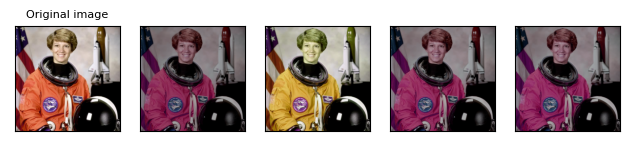
\includegraphics[width=1\textwidth]{figs/jitter.png}
    \caption{ColorJitter augmentation example \cite{colorjitter}}
    \label{jitter}
\end{figure}

Our best model with data augmented by ColorJitter, on $4\,000$ labeled datapoints and $46\,000$ unlabeled datapoints and learning rate $0.5$ achieved accuracy \textbf{91\%}, which is not better than with the same hyperparameters and only flip and rotate augmentations. Based on this result, in further experimenting, we used only flip and rotate augmentations.





\subsection{Experiment 3: Portion of labeled data}

In this final experiment, we tended to investigate how unlabeled data support the model in cases when a very limited portion of labeled samples is used.
In the original Binary mean teacher paper, Tuna et al.\cite{tuna-bmt} focused on setups with $8\%$ and $1\%$ labeled samples in the training set. We focused on even smaller portions.

We denote a new hyperparameter portion of labeled data as $P$. In our experiments, we tried values of $P = 4\,000, 1\,000, 500, 100$. For each value of $P$, we tried, based on Experiment 1 results, two best values of learning rate (LR). The complete results are shown in Table \ref{portions}. Values in the second column mean the percentage of labeled data in the training set. Highlighted results show cases when the Binary Mean Teacher model achieved better accuracy than the baseline model.

\bigskip

\begin{table}[h]
    \centering
    \begin{tabular}{ |c|c|c|c|c|} 
     \hline

     P & \% labeled & LR & Student test accuracy & Baseline test accuract\\
     \hline
     
     100 & 0.2\%& 0.1 & \color{purple}  78\%   &  60\% \\ 
     \hline
     100 & 0.2\% & 0.5 & \color{purple} 80\%  & 60\% \\
     \hline
     500 & 1\% & 0.5 & \color{purple} 88\% &  85\% \\
     \hline
     500 & 1\% & 0.1 & \color{purple} 88\% &  85\% \\
     \hline
     1000 & 2\% & 0.1 & \color{purple}89\% &  83\% \\
     \hline
     1000 & 2\% & 0.5 & \color{purple}90\% &  83\%  \\
     \hline
     4000 & 8\% & 0.1 & 89\% & 93\% \\
     \hline
     4000 & 8\% & 0.5 & 91\% & 93\%  \\
     
     \hline
    \end{tabular}
    \caption{Comparison of model test accuracy}
    \label{portions}
\end{table}


\section{Discussion of results} 
The first experiment showed, that $4000$ labeled samples are enough for the supervised model to train well ($93\%$). The semi-supervised model didn't achieve this high accuracy even when trying different values of the learning rate hyperparameter.

In the second experiment, we tried to use different augmentation - a change of colors in the image. In this case, the model did not work any better than using only flip and rotation. Accuracy stayed the same.


The last experiment focused on how different portions of labeled data influenced the model's accuracy. This experiment showed that the semi-supervised model worked much better for smaller portions of data, in cases when the supervised model wasn't able to accomplish that high accuracy. This experiment showed, that huge unlabeled samples used for training of semi-supervised model helped its performance.

There are several things about the Binary Mean Teacher model, that could be studied in the future. We recommend future research to focus on more complex architectures, which was not possible for us, because of our hardware limitations. The study of different hyperparameters, such as EMA decay or consistency cost weight in the weighted sum of costs could also help to reach better performance.


